\documentclass[a4paper,10pt]{article}

\usepackage[T1]{fontenc}
\usepackage[utf8]{inputenc}
\usepackage[english]{babel}
\usepackage[a4paper, top=2cm, bottom=2cm, left=2cm, right=2cm]{geometry}
\usepackage{lmodern}
\usepackage{booktabs}
\usepackage{xcolor}
\usepackage{pgfplots}
\pgfplotsset{compat=1.18}
\usepackage{tikz}
\usetikzlibrary{arrows.meta, positioning, fit, backgrounds}
\usepackage{microtype}
\usepackage{parskip}
\usepackage{enumitem}
\usepackage{amssymb}
\setlength{\parskip}{3pt}
\setlength{\parindent}{0pt}

\definecolor{c1}{RGB}{31,119,180}
\definecolor{c2}{RGB}{44,160,44}
\definecolor{c3}{RGB}{255,127,14}
\definecolor{c4}{RGB}{148,103,189}
\definecolor{c5}{RGB}{214,39,40}
\definecolor{c6}{RGB}{23,190,207}
\definecolor{lightgray}{RGB}{245,245,245}

\newcommand{\slide}[2]{%
  \item[$\square$] \textbf{#1} \quad {\small #2}%
}

\captionsetup{font=small, labelfont=bf}

\title{\textbf{Proposed Presentation Structure}\\[0.2em]
{\normalsize Mitigating Time-Shift Errors in CGM-based Glucose Forecasting\\
and Hypoglycemia Event Prediction}}
\author{Robin van den Hoek\quad|\quad PRG Seminar, University of Bern}
\date{Talk date: TBD\quad|\quad Duration: $\approx$30 min + Q\&A\quad|\quad Tool: \LaTeX/Beamer}

\begin{document}
\maketitle
\vspace{-1em}
\hrule
\vspace{0.5em}

{\small\textit{Use this document to mark which slides to \textbf{keep}, \textbf{shorten}, or \textbf{drop} during the meeting. Legend: $\square$ = undecided \quad $\checkmark$ = keep \quad $\times$ = drop/shorten.}}

\vspace{0.6em}

% ─────────────────────────────────────────────────────────────────────────────
% Overview diagram
% ─────────────────────────────────────────────────────────────────────────────

\begin{figure}[h!]
\centering
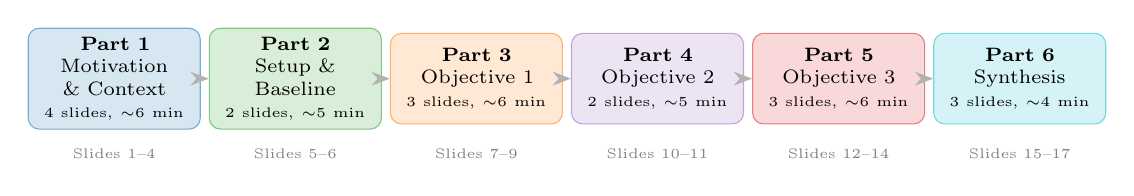
\begin{tikzpicture}[
  part/.style={draw, rounded corners=4pt, minimum width=2.05cm, minimum height=1.15cm,
               align=center, font=\scriptsize, text width=1.95cm},
  arr/.style={->, >=Stealth, thick, gray!60}
]
\node[part, fill=c1!18, draw=c1!60]  (p1) at (0,0)
  {\textbf{Part 1}\\Motivation \& Context\\{\tiny 4 slides, $\sim$6 min}};

\node[part, fill=c2!18, draw=c2!60]  (p2) at (2.3,0)
  {\textbf{Part 2}\\Setup \& Baseline\\{\tiny 2 slides, $\sim$5 min}};

\node[part, fill=c3!18, draw=c3!60]  (p3) at (4.6,0)
  {\textbf{Part 3}\\Objective 1\\{\tiny 3 slides, $\sim$6 min}};

\node[part, fill=c4!18, draw=c4!60]  (p4) at (6.9,0)
  {\textbf{Part 4}\\Objective 2\\{\tiny 2 slides, $\sim$5 min}};

\node[part, fill=c5!18, draw=c5!60]  (p5) at (9.2,0)
  {\textbf{Part 5}\\Objective 3\\{\tiny 3 slides, $\sim$6 min}};

\node[part, fill=c6!18, draw=c6!60]  (p6) at (11.5,0)
  {\textbf{Part 6}\\Synthesis\\{\tiny 3 slides, $\sim$4 min}};

\foreach \a/\b in {p1/p2, p2/p3, p3/p4, p4/p5, p5/p6}
  \draw[arr] (\a.east) -- (\b.west);

\node[font=\tiny, gray] at (0,-0.95) {Slides 1--4};
\node[font=\tiny, gray] at (2.3,-0.95) {Slides 5--6};
\node[font=\tiny, gray] at (4.6,-0.95) {Slides 7--9};
\node[font=\tiny, gray] at (6.9,-0.95) {Slides 10--11};
\node[font=\tiny, gray] at (9.2,-0.95) {Slides 12--14};
\node[font=\tiny, gray] at (11.5,-0.95) {Slides 15--17};
\end{tikzpicture}
\caption{Presentation overview: 17 slides, $\approx$30 min. Slide numbers are indicative --- adjust based on meeting decisions.}
\end{figure}

\vspace{-0.3em}

% ─────────────────────────────────────────────────────────────────────────────
\section*{\textcolor{c1!80!black}{Part 1 --- Motivation \& Context} \hfill\small $\sim$6 min, 4 slides}
% ─────────────────────────────────────────────────────────────────────────────

\begin{itemize}[leftmargin=1.8em, itemsep=2pt]
\slide{Title slide}{Thesis title, name, supervisor, date. One-sentence problem statement.}
\slide{Clinical motivation}{CGM devices, Type 1 diabetes, hypoglycemia danger. Key question: what does a 55-min prediction lag mean for a patient who needs to eat carbohydrates in time?}
\slide{The time-shift problem}{Figure: glucose curve overlaid with shifted prediction. Introduce lag\_rmse as the metric isolating the shift component. Key message: MSE-trained models reproduce the right shape, but always too late.}
\slide{Related work \& positioning}{Hüni (2023): LSTM vs.\ GAT for hypoglycemia prediction at University of Bern. This thesis: same dataset, same evaluation protocol --- three systematic mitigations, controlled ablation (one factor at a time).}
\end{itemize}

% ─────────────────────────────────────────────────────────────────────────────
\section*{\textcolor{c2!70!black}{Part 2 --- Experimental Setup \& Baseline} \hfill\small $\sim$5 min, 2 slides}
% ─────────────────────────────────────────────────────────────────────────────

\begin{itemize}[leftmargin=1.8em, itemsep=2pt]
\slide{Experimental setup}{36 patients, 5-min intervals, lookback\,=\,24 steps (2\,h), horizon $h{=}11$ (60 min). Train/Val/Test: 60/20/20 temporal split per patient, 36 patient-specific models. Architectures: LSTM and PatchTST. HP tuning: Optuna on patient 85202; all objectives reuse same HP.}
\slide{Baseline results}{Table: LSTM RMSE\,=\,36.09, PatchTST RMSE\,=\,39.27; both $F_1 \approx 0$. Mean shift: LSTM 10.2 steps (51 min), PatchTST 11.0 steps (55 min). Key message: MSE training fails at event detection --- motivates all three objectives.}
\end{itemize}

% ─────────────────────────────────────────────────────────────────────────────
\section*{\textcolor{c3!80!black}{Part 3 --- Objective 1: Offset-Aware Losses} \hfill\small $\sim$6 min, 3 slides}
% ─────────────────────────────────────────────────────────────────────────────

\begin{itemize}[leftmargin=1.8em, itemsep=2pt]
\slide{Objective 1a: Bounded-Lag loss}{Formula: $L = \min_{\Delta \in [-3,3]} \mathrm{MSE}(\hat{y}, y_\Delta)$. $D{=}3$ steps ($\pm$15 min): within this window, temporal alignment is free. Results: RMSE negligible change ($\Delta{<}0.05$ mg/dL); PatchTST lag\_rmse\,=\,16.70 (best of Obj.\ 1); slight $F_1$ improvement for LSTM (0.005 $\to$ 0.014).}
\slide{Objective 1b: Soft-DTW loss}{Differentiable DTW with $\gamma{=}1.0$; allows elastic alignment along the full sequence path. Results: RMSE regression (+1.1 LSTM, +3.96 PatchTST mg/dL); higher lag\_rmse than Bounded-Lag. DTW deprioritises exact amplitude --- direct conflict with RMSE evaluation metric.}
\slide{Objective 1 conclusion}{Summary table for all 4 model-loss combinations. Key message: $D{=}3$ covers only $\approx$30\% of the actual shift; loss relaxation reduces training penalty but does not provide structural information to predict earlier. Transition: $\to$ Objective 2 (multi-step supervision).}
\end{itemize}

% ─────────────────────────────────────────────────────────────────────────────
\section*{\textcolor{c4!80!black}{Part 4 --- Objective 2: Multi-Step Forecasting} \hfill\small $\sim$5 min, 2 slides}
% ─────────────────────────────────────────────────────────────────────────────

\begin{itemize}[leftmargin=1.8em, itemsep=2pt]
\slide{Multi-step concept (DIRMO)}{Model outputs all 12 steps simultaneously; loss averaged over full trajectory. Hypothesis: predicting intermediate steps keeps the model ``in phase'' over the full horizon. Evaluation still at $h{=}11$ for fair comparison.}
\slide{Multi-step results}{Bar chart: RMSE and lag\_rmse comparison. LSTM: RMSE\,=\,35.59 ($-0.50$), lag\_rmse\,=\,20.74; PatchTST: RMSE\,=\,39.05 ($-0.22$), lag\_rmse\,=\,14.53. Key message: \textbf{lowest lag\_rmse of any tested method} --- but shift penalty remains 40--63\% of RMSE.}
\end{itemize}

% ─────────────────────────────────────────────────────────────────────────────
\section*{\textcolor{c5!80!black}{Part 5 --- Objective 3: Event-Centric} \hfill\small $\sim$6 min, 3 slides}
% ─────────────────────────────────────────────────────────────────────────────

\begin{itemize}[leftmargin=1.8em, itemsep=2pt]
\slide{$\tau$-sweep: cost of the shift}{Plot: $F_1$ vs.\ tolerance $\tau$ (0--12 steps) for all forecasting models. Key message: all forecasting models require $\tau{>}5$ steps (25 min) for non-trivial recall. At $\tau{=}3$ (15 min, clinically appropriate), forecast-derived detection fails.}
\slide{Direct binary event classifier}{Architecture: same LSTM/PatchTST, sigmoid output head, BCE loss. Label: 1 if any $y_{t:t+12} < 70$ mg/dL. Results: LSTM $F_1{=}0.334$ (\textbf{62$\times$ improvement} over baseline $F_1{=}0.005$), Recall\,=\,69\%. PatchTST: $F_1{=}0.095$, very high false positive rate (Precision\,=\,0.054).}
\slide{Objective 3 conclusion: architecture inversion}{Table: LSTM vs.\ PatchTST across forecasting and classification. LSTM is worse at forecasting (RMSE 36.09 vs.\ 39.27) but 3.5$\times$ better at event classification ($F_1$ 0.334 vs.\ 0.095). Key message: recurrent state tracking suits binary event prediction; the two tasks must be separated.}
\end{itemize}

% ─────────────────────────────────────────────────────────────────────────────
\section*{\textcolor{c6!70!black}{Part 6 --- Synthesis \& Close} \hfill\small $\sim$4 min, 3 slides}
% ─────────────────────────────────────────────────────────────────────────────

\begin{itemize}[leftmargin=1.8em, itemsep=2pt]
\slide{Overall comparison \& recommendation}{Full comparison table (all methods $\times$ RMSE/lag\_rmse/$F_1$). Recommendation: Multi-step MSE for glucose trajectory; LSTM binary classifier for hypoglycemia warning. Consistent with Hüni (2023): treat forecasting and event prediction as separate tasks.}
\slide{Limitations \& future work}{$D{=}3$ window too narrow for a 50-min shift; larger window unexplored. Class imbalance: LSTM precision still 0.237 (1 in 4 alarms is real). Optional Objective 4: post-hoc shift correction ($k^*$ subtracted at inference). Per-patient RMSE std $\approx$7--8 mg/dL --- personalisation unexplored.}
\slide{Discussion questions}{\textbf{Q1:} The Bounded-Lag window $D{=}3$ covers only 30\% of the observed shift. Would a larger window (e.g.\ $D{=}6$ or $D{=}11$) be worth exploring, and where would you set the bound? \quad \textbf{Q2:} The LSTM event classifier achieves Recall\,=\,0.69 but Precision\,=\,0.24 (3 in 4 alarms are false). Is this acceptable for a clinical alert system, and how should the threshold be calibrated?}
\end{itemize}

\begin{itemize}[leftmargin=1.8em, itemsep=2pt]
\slide{References}{One slide listing cited works (Hüni 2023, Cuturi \& Blondel 2017, Sakoe \& Chiba 1978, relevant LSTM/PatchTST papers).}
\end{itemize}

\vspace{0.5em}
\hrule
\vspace{0.5em}

% ─────────────────────────────────────────────────────────────────────────────
\section*{Time Budget}
% ─────────────────────────────────────────────────────────────────────────────

\begin{center}
\begin{tabular}{llcc}
\toprule
Part & Topic & Slides & Time \\
\midrule
1 & Motivation \& Context    & 4 & $\sim$6 min \\
2 & Setup \& Baseline        & 2 & $\sim$5 min \\
3 & Objective 1 (Losses)     & 3 & $\sim$6 min \\
4 & Objective 2 (Multi-step) & 2 & $\sim$5 min \\
5 & Objective 3 (Events)     & 3 & $\sim$6 min \\
6 & Synthesis \& Close       & 3 & $\sim$4 min \\
  & References               & 1 & --- \\
\midrule
\textbf{Total} & & \textbf{18} & \textbf{$\approx$32 min} \\
\bottomrule
\end{tabular}
\end{center}

\vspace{0.8em}

% ─────────────────────────────────────────────────────────────────────────────
\section*{Notes from Meeting}
% ─────────────────────────────────────────────────────────────────────────────

\vspace{4cm}

\hrule

\end{document}
